\documentclass{eage2020}

\usepackage{subfig}

\usepackage[UKenglish]{babel}
\usepackage[utf8]{inputenc}
\usepackage{lmodern}
\usepackage[T1]{fontenc}
\usepackage[pdftex, hidelinks]{hyperref}

\usepackage{xspace}
\usepackage{siunitx}
\newcommand{\mr}[1]{\mathrm{#1}}
\newcommand{\emg}[2]{\texttt{emg#1#2}\xspace}
\newcommand{\empymod}{\texttt{empymod}\xspace}

\graphicspath{{./figures/}}

\begin{document}

\section{Introduction}

Controlled-source electromagnetic (CSEM) methods have been used since decades
in exploration geophysics, with a major hype in the early 2000s in the oil
industry. These days it is one of the many established, non-seismic methods in
the exploration of resources in the subsurface, not just for hydrocarbons but
also for water and geothermal resources, mining, and civil engineering tasks.
As a consequence various 3D CSEM codes have been developed since a long time,
e.g. \cite{B.SEG.99.Oristaglio}. However, they were often proprietary or only
available upon request from the author. Recently it has become possible to
install different 3D CSEM modellers with a single command in the Python
ecosystem, e.g., SimPEG \citep{SimPEG}, PETGEM \citep{PETGEM}, custEM
\citep{custEM}, or emg3d \citep{JOSS.19.Werthmuller}. This, together with
increased computing power, makes it possible for anyone to compute CSEM
responses for realistic real-world models. We tried to speed-up the computation
of time-domain responses with a frequency-domain code by (a) improving existing
methods, and (b) computing in the real-valued Laplace domain instead of the
complex-valued frequency domain. While the former idea works fine the latter
idea does only work with exact arithmetic results but unfortunately not when
numerical approximations must be made.

For the 1D computations and for designing digital linear filters we use
\empymod \citep{GEO.17.Werthmuller}, and for the 3D computation we use the
multigrid code \emg3d \citep{JOSS.19.Werthmuller}; both codes are released
under the Apache License 2.0 and can be found on
\href{https://empymod.github.io}{empymod.github.io}. The multigrid solver
\emg3d solves the diffusive approximation of Maxwell's equation given by the
second-order differential equation of the electric field,
%
\begin{equation}
    s\mu_0 \sigma \mathbf{E} -
    \nabla \times \mu_\mr{r}^{-1} \nabla \times \mathbf{E}
    = -s\mu_0 \mathbf{J}_\mathrm{s} \, ,
  \label{eq:maxwell}
\end{equation}
%
where $\sigma$ is conductivity (S/m), $s=\mr{i}\omega$ is the Laplace parameter
and $\omega=2\pi f$ is angular frequency of frequency $f$ (Hz),
$\mu=\mu_0\mu_\mr{r}$ is magnetic permeability (H/m), $\mathbf{E}$ is the
electric field (V/m), and $\mathbf{J}_\mathrm{s}$ the current source (A/m$^2$).
The diffusive approximation neglects displacement currents by assuming that
$\omega\varepsilon \ll \sigma$, where $\varepsilon$ is electric permittivity
(F/m). The advantage of a matrix-free multigrid solver is that it scales
linearly with the number of cells for both CPU and RAM usage
\citep{B.Springer.11.Mulder}. All examples shown here were computed on a laptop
with an i7-6600U\,CPU\,@\,2.6\,GHz (x4) and 16\,GB of memory, using Ubuntu
18.04 and Python 3.7.

\section{Time-domain modelling with a frequency-domain code}

Computing time-domain data with a frequency-domain code requires the
computation of a range of frequencies as input for the Fourier transform; for
marine CSEM roughly from 0.001\,Hz to 100\,Hz (depending on the required offset
one can get away with a much smaller range). The required computation grids
vary a lot from low to high frequencies. An automatic, adaptive gridding scheme
is therefore required, which is usually based on the skin depth
$\delta\approx503.3/\sqrt{f\sigma}$, the depth after which the signal
attenuated to $1/e\approx 37\,\%$.

Our scheme is based on the automatic gridding as suggested by
\cite{GEO.07.Plessix}, and the adaptive frequency selection as presented by
\cite{GEO.08.Mulder}. Making two changes to their schemes resulted in
substantial, model-dependent speed-up. The major change lies in the automatic
gridding. Instead of looking for the optimal parameters (minimum cell width,
stretching factor, domain size) for a given number of cells in each direction
we are looking for the minimal number of cells required which still comply with
the ranges we define for these parameters. Using a Fourier transform that works
with logarithmically spaced values, such as digital linear filters \citep[DLF,
][]{GP.71.Ghosh} or the logarithmic fast Fourier transform \citep[FFTLog,
][]{RAS.00.Hamilton} further improved the overall speed. Carefully selecting
the frequency-range showed that 20 frequencies or less are often sufficient for
a wide range of offsets.

Figure \ref{fig:fullspace} shows an example, where we reproduced the fullspace
model of \cite{GEO.08.Mulder} in less than 2 minutes, while their original
computation took roughly 3.75 hours. The model is a homogeneous fullspace of
1\,S/m, an $x$-directed source at the origin, 1\,Hz, and an $x$-directed inline
receiver at an offset of 900\,m. We defined the FFTLog with 30 frequencies,
$0.0002-126\,$Hz, but actually required to compute are only 14 frequencies,
$0.05-20\,$Hz (blue circles in the figure). Responses for $f>20\,$Hz were set
to zero and responses for $f<0.05\,$Hz were interpolated by assuming that the
imaginary part of $E_x$ goes linearly to zero in log-frequency scale.
%
\begin{figure}[tb]
  \centering
  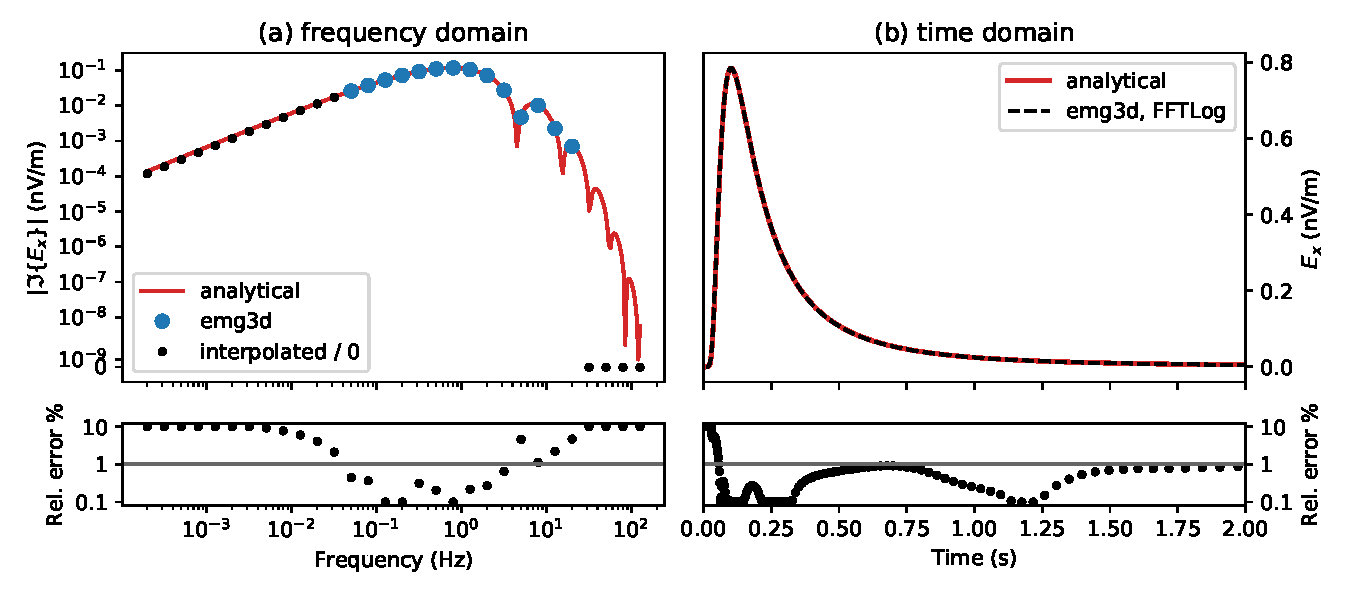
\includegraphics[width=\textwidth]{fullspace}
  \caption{(a) Imaginary frequency-domain response, where the blue circles are
    computed with \emg3d, and the black dots are interpolated or set to 0. (b)
    Corresponding time-domain response. The errors are clipped at $[0.1,
    10]$\,\%}
  \label{fig:fullspace}
\end{figure}
%

The time-domain result is shown in Figure \ref{fig:fullspace}b, where it can be
seen that the relative error is always below 1\,\%, except for very early
times. The frequency selection is important for the speed-up, as our scheme
only required 14 frequencies in comparison to the 26 frequencies computed in
the original publication. However, the most important change in terms of speed
is in the adaptive gridding.


\section{Laplace-domain computation}

The complex-valued Laplace parameter $s=\mr{i}\omega$ can be replaced with a
real-valued $s$ to compute CSEM data in the space-Laplace domain instead of the
space-frequency domain. Figure~\ref{fig:motivation} shows a comparison of
space-frequency and space-Laplace domain computations. The model is a diffusive
halfspace with $x$-directed source and receiver, where the source is at 500\,m
depth, and the receiver at $x=y=1\,$km at a depth of 600\,m; subsurface
conductivity is 1\,S/m. There are two main motivations to use Laplace-domain
computations: (a) real-valued instead of complex operations, and (b) smoother,
non-oscillating responses. The former should result in faster computation times
of a single solver iteration, the latter is expected to result in faster
convergence.
%
\begin{figure}[tb]
  \centering
  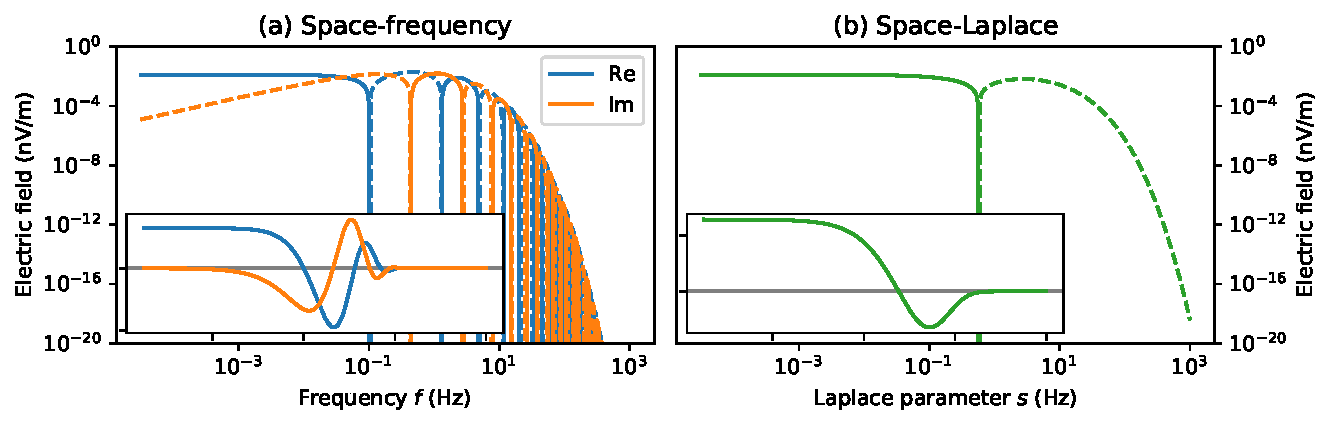
\includegraphics[width=\textwidth]{motivationcomparison}
  \caption{Comparison of a CSEM response in (a) the space-frequency and in (b)
    the space-Laplace domain; the inset figures show the same but with a linear
    scale for the y-axis. The motivation for Laplace-domain computations is
    real-valued operations and no oscillating behaviour in comparison to
    frequency-domain responses.}
  \label{fig:motivation}
\end{figure}
%

We implemented the possibility of space-Laplace domain computations into both
\empymod (v1.9.0) and \emg3d (v0.8.0). To test if Laplace-domain computations
are faster than frequency-domain computations we run a complex, isotropic model
with roughly 2.1 million cells in both domains, as shown in
Figure~\ref{fig:sLtime}. We chose a frequency of 1\,Hz, which yields in the
frequency domain $\rm{i}\omega=\rm{i}2\pi f$ and in the Laplace domain we took
the equivalent of $s=2\pi f$. An average iteration in the space-frequency
domain took 9.9 seconds, and 16 multigrid cycles were required to reach the
desired tolerance. In the space-Laplace domain it took 8.0 seconds per
iteration, and 14 multigrid cycles were required. So both expectations, faster
computation and faster convergence, could be confirmed. The overall speed-up in
this case is a factor of 0.71.
%
\begin{figure}[b]%
  \centering
  \parbox{.48\linewidth}{
    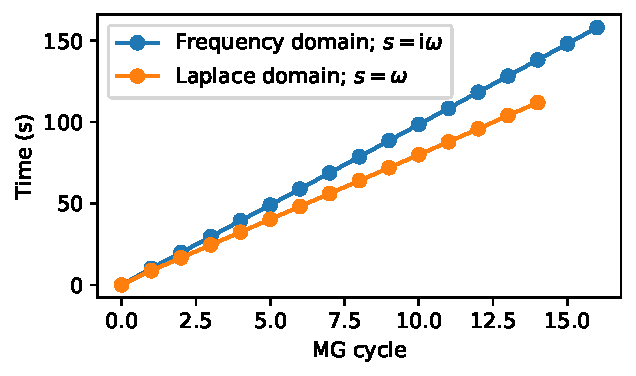
\includegraphics[width=\linewidth]{xf-vs-xs}%
    \caption{Runtime comparison between space-frequency and space-Laplace
      domain computations. The space-Laplace domain computation is faster per
      cycle and requires less cycles.}
    \label{fig:sLtime}
  }
  \hfill
  \begin{minipage}{.48\linewidth}%
    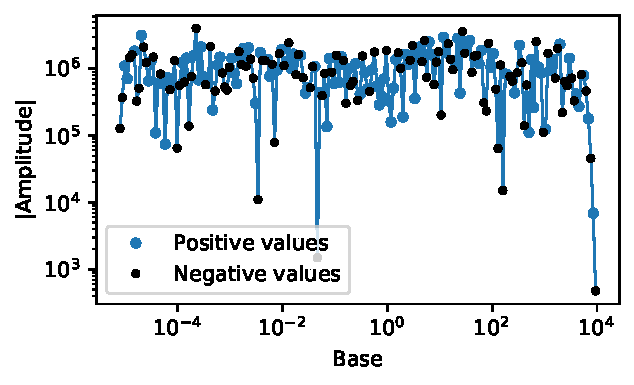
\includegraphics[width=\linewidth]{filter-space}%
    \caption{The derived 201\,pt Laplace filter using the
      \texttt{fdesign}-routine of \empymod with the analytical Laplace- and
      time-domain functions as input values.}
    \label{fig:LaplaceDLF}
  \end{minipage}
\end{figure}
%

There is no analytical transformation from the Laplace domain to the time
domain. However, we were able to derive a digital linear filter for the
Laplace-to-time transformation using the \texttt{fdesign}-routine of \empymod
and the analytical Laplace- and time-domain functions as input values. The
filter is shown in Figure ~\ref{fig:LaplaceDLF}, and a show-case of the filter
in Figure ~\ref{fig:s-t_time}a. The model is a diffusive, $x$-directed impulse
response, inline, of a halfspace of 1\,S/m conductivity and vertical transverse
conductivity of $\sqrt{2}$. The source is located at the origin at a depth of
150\,m, the receiver is at an offset of 2\,km at a depth of 200\,m. The
time-domain result obtained through Laplace-domain computation followed by a
DLF yields the time-domain response accurately.
%
\begin{figure}[tb]
  \centering
  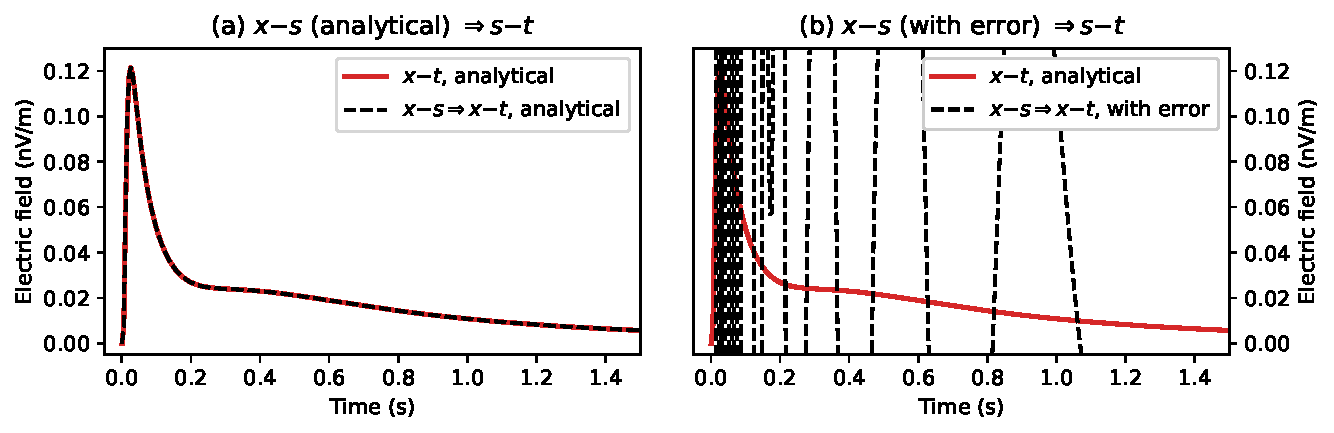
\includegraphics[width=\linewidth]{s-t_time}%
  \caption{(a) Laplace-to-time DLF works fine for analytical responses. (b) As
    soon as the Laplace-domain has the slightest error it fails. The red curve,
    the analytical time-domain result, is the same in both plots.}
  \label{fig:s-t_time}
\end{figure}
%

Given these encouraging initial results we tried to apply it to 3D modelling
results, however, without success. We therefore returned again to 1D modelling
to analyze the problem: Figure~\ref{fig:s-t_time}b shows the exactly same data
as Figure \ref{fig:s-t_time}a. The only difference is that we multiplied the
amplitude of $s=7.043$ by 1.00001. This tiny error causes the whole DLF to
fail.

\section{Conclusions}

We have shown that computing 3D time-domain CSEM data with computation in the
frequency domain is very competitive if (a) the frequency-dependent adaptive
gridding is optimized to use as few cells as possible and (b) a
logarithmically-scaled Fourier transform is used such as DLF or FFTLog, with
careful frequency selection. Computation in the Laplace domain results in
faster computation time (real vs. complex operations) and faster convergence
(smoother behaviour) when compared with computation in the frequency domain.
However, using Laplace-domain computations to obtain time-domain CSEM responses
fails, as the Laplace-DLF requires very precise and complete input data, unlike
the sine- or cosine-DLF for the Fourier transform.

\section{Acknowledgements}

This research was conducted within the Gitaro.JIM project funded through
MarTERA, a EU Horizon 2020 research and innovation programme (No 728053);
\href{https://www.martera.eu}{martera.eu}.

\begin{thebibliography}{11}
\providecommand{\natexlab}[1]{#1}

\bibitem[Castillo-Reyes et~al., 2018]{PETGEM}
Castillo-Reyes, O., de~la Puente, J. and Cela, J.M. [2018] {PETGEM}: {A}
  parallel code for {3D} {CSEM} forward modeling using edge finite elements.
\newblock \emph{Computers \& Geosciences}, \textbf{119}, 123--136.
\newblock \href{https://doi.org/10.1016/j.cageo.2018.07.005}{DOI:
  10.1016/j.cageo.2018.07.005}.

\bibitem[Cockett et~al., 2015]{SimPEG}
Cockett, R., Kang, S., Heagy, L.J., Pidlisecky, A. and Oldenburg, D.W. [2015]
  {SimPEG}: {A}n open source framework for simulation and gradient based
  parameter estimation in geophysical applications.
\newblock \emph{Computers \& Geosciences}, \textbf{85}, 142--154.
\newblock \href{https://doi.org/10.1016/j.cageo.2015.09.015}{DOI:
    10.1016/j.cageo.2015.09.015}.

\bibitem[Ghosh, 1971]{GP.71.Ghosh}
Ghosh, D.P. [1971] The application of linear filter theory to the direct
  interpretation of geoelectrical resistivity sounding measurements.
\newblock \textbf{19}(2), 192--217.
\newblock \href{https://doi.org/10.1111/j.1365-2478.1971.tb00593.x}{DOI:
  10.1111/j.1365-2478.1971.tb00593.x}.

\bibitem[Hamilton, 2000]{RAS.00.Hamilton}
Hamilton, A.J.S. [2000] Uncorrelated modes of the non-linear power spectrum.
\newblock \emph{Monthly Notices of the Royal Astronomical Society},
  \textbf{312}(2), 257--284.
\newblock \href{https://doi.org/10.1046/j.1365-8711.2000.03071.x}{DOI:
  10.1046/j.1365-8711.2000.03071.x}.

\bibitem[Mulder, 2011]{B.Springer.11.Mulder}
Mulder, W.A. [2011] \emph{Numerical Methods, Multigrid}.
\newblock Springer Netherlands, Dordrecht, 895--900.
\newblock \href{https://doi.org/10.1007/978-90-481-8702-7_153}{DOI:
  10.1007/978-90-481-8702-7\_153}.

\bibitem[Mulder et~al., 2008]{GEO.08.Mulder}
Mulder, W.A., Wirianto, M. and Slob, E. [2008] Time-domain modeling of
  electromagnetic diffusion with a frequency-domain code.
\newblock \emph{Geophysics}, \textbf{73}(1), F1--F8.
\newblock \href{https://doi.org/10.1190/1.2799093}{DOI: 10.1190/1.2799093}.

\bibitem[Oristaglio and Spies, 1999]{B.SEG.99.Oristaglio}
Oristaglio, M. and Spies, B. (Eds.)  [1999] \emph{Three-Dimensional
  Electromagnetics}.
\newblock No.~7 in Geophysical Developments. SEG.
\newblock \href{https://doi.org/10.1190/1.9781560802154}{DOI:
  10.1190/1.9781560802154}.

\bibitem[Plessix et~al., 2007]{GEO.07.Plessix}
Plessix, R.E., Darnet, M. and Mulder, W.A. [2007] An approach for {3D}
  multisource, multifrequency {CSEM} modeling.
\newblock \emph{Geophysics}, \textbf{72}(5), SM177--SM184.
\newblock \href{https://doi.org/10.1190/1.2744234}{DOI: 10.1190/1.2744234}.

\bibitem[Rochlitz et~al., 2019]{custEM}
Rochlitz, R., Skibbe, N. and Günther, T. [2019] {custEM}: customizable finite
  element simulation of complex controlled-source electromagnetic data.
\newblock \emph{Geophysics}, \textbf{84}(2), F17--F33.
\newblock \href{https://doi.org/10.1190/geo2018-0208.1}{DOI:
  10.1190/geo2018-0208.1}.

\bibitem[Werthmüller, 2017]{GEO.17.Werthmuller}
Werthmüller, D. [2017] An open-source full {3D} electromagnetic modeler for
  {1D} {VTI} media in {P}ython: empymod.
\newblock \emph{Geophysics}, \textbf{82}(6), WB9--WB19.
\newblock \href{https://doi.org/10.1190/geo2016-0626.1}{DOI:
  10.1190/geo2016-0626.1}.

\bibitem[Werthmüller et~al., 2019]{JOSS.19.Werthmuller}
Werthmüller, D., Mulder, W.A. and Slob, E.C. [2019] {e}mg3d: {A} multigrid
  solver for {3D} electromagnetic diffusion.
\newblock \emph{Journal of Open Source Software}, \textbf{4}(39), 1463.
\newblock \href{https://doi.org/10.21105/joss.01463}{DOI: 10.21105/joss.01463}.

\end{thebibliography}

\end{document}
